A figura \ref{module} apresenta a estrutura de módulos (a fim de evitar poluição visual, as relações serão apresentadas
em outra figura). 

\begin{figure}[H]
  \centering
  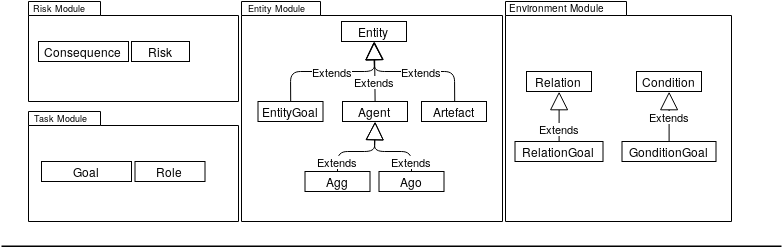
\includegraphics[width=1\linewidth]{figure/Module.png} 
  \caption{A estrutura geral das classes do modelo}
  \label{module}
\end{figure}

Assim sendo, assumindo que existe $\Omega_{Model}$ (um conjunto global onde todos os outros conjuntos do modelo estão 
contidos nele), os módulos são representados da seguinte maneira; 

\begin{equation} 
    \Omega_{Model} = \{ M_{Risk}, M_{Task}, M_{Entity}, M_{Environment}\}
\end{equation}
\label{modules}
